\documentclass[a4paper]{article}

\usepackage[margin=1cm]{geometry}

\usepackage{graphicx}
\usepackage{tabularx}
\usepackage{tikz}
\usetikzlibrary{calc,positioning,shapes.geometric,arrows.meta,fit}
\pagestyle{empty}

\usepackage[utf8x]{inputenc}

\usepackage[english]{babel}

\usepackage{parskip}
\usepackage{pxfonts}

%\usepackage[active,tightpage]{preview}
%\setlength{\PreviewBorder}{10pt}
%\PreviewEnvironment{tikzpicture}

\newcommand{\s}[1]{{\bfseries\Large #1}}

\newcommand{\im}[1]{
\begin{tikzpicture}[xscale=2.3,yscale=2.3]

\foreach \a in {1,2,...,6}{
\node (x\a) [circle, fill=black, inner sep=2pt, outer sep=2pt] at (360-\a*360/6: 1cm) {};%TCZ $\a$};
}

\draw [line width=0pt] (x1) -- node [midway, below=5mm] {mouse 1} (x2);
\draw [line width=0pt] (x3) -- node [midway, above=5mm,sloped] {mouse 2} (x4);
\draw [line width=0pt] (x5) -- node [midway, above=5mm,sloped] {mouse 3} (x6);

#1

\end{tikzpicture}
}

\renewcommand{\familydefault}{\sfdefault}


\begin{document}

\sffamily

\begin{tabular}{lll}
\s{a} & \s{b} & \s{c}  \\
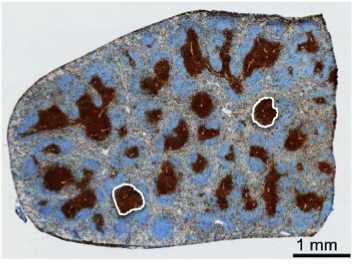
\includegraphics[angle=0,height=2.4in]{images/spleen.png} &
	{\includegraphics[page=1]{plots/basic.pdf}} &
\includegraphics[page=2]{plots/basic.pdf} \\
%\includegraphics[page=3]{plots/p.pdf} \\
%\s{e} \\
%\includegraphics[page=4]{plots/p.pdf} 
\end{tabular}

\begin{tabular}{lll}
\s{d} & \s{e} & \s{f} \\
\includegraphics[page=1]{plots/clonefreq.pdf} & 
\includegraphics[page=1]{plots/vdist.pdf} & 
\includegraphics[page=1]{plots/jdist.pdf}
\end{tabular}

{\bfseries Figure 1: Interrogating the local repertoire in splenic T cell zones in mice.} (a) Cross-section of a murine spleen with two separate T cell zones (TCZs) highlighted. (b) Number of reads mapped to the CDR3$\beta$ region for six TCZs in three mice. (c) Number of unique productive CDR3$\beta$ amino acid sequences extracted from the reads in (b). (d) Distribution of mapped reads per clone. (e, f) Overview of (e) V gene and (f) J gene usage within each sample.

\newpage

\begin{tabular}{lll}
\s{a} & \s{b} & \s{c} \\[-1em]
\includegraphics[page=1]{plots/fig2.pdf} & 
{\includegraphics[page=1]{plots/reads-shared.pdf}} & 
\includegraphics[page=2]{plots/reads-shared.pdf}
\end{tabular}


\begin{tabular}{l}
\s{d} \\[-1em]
\includegraphics[page=1]{plots/usage-shared.pdf}
\end{tabular}
%\includegraphics[page=2]{plots/usage-shared.pdf}

\begin{tabular}{l}
\s{e} \\[-1em]
\includegraphics[page=2]{plots/usage-shared.pdf}
\end{tabular}

\begin{tabular}{ll}
\s{f} & \s{g} \\[-1em]
\includegraphics[page=1]{plots/vjnuc.pdf} & 
\includegraphics[page=2]{plots/vjnuc.pdf}
\end{tabular}

{\bf Figure 2: TCZ repertoire overlap is similar within and between mice, and related to precursor frequency.} (a) Jaccard index (percentage of clones in the pooled sample occurring in both samples) for each pair of TCZs. (b, c) Number of reads for shared and unique clones on the within-mouse (b) and between-mouse levels (c). Boxplots show medians and interquartile ranges, whiskers show minima and maxima. (d) V and J gene usage for reads whose TCR sequence is shared or not shared (unique) between two TCZs of the same mouse. Error bars depict 95\% confidence intervals (CIs). (e) V and J gene usage of reads shared or not shared between each pair of mice after pooling the reads from the two TCZs of each mouse. Error bars: 95\% CIs. (f) Distributions of the distance in number of nucleotides between the end of the mapped V segment and the beginning of the mapped J segment. Arrows depict means. (g) Distribution of the number of nucleotides between V and J in each read that cannot be mapped to a D segment. Arrows depict means.

\newpage

\begin{tabular}{lrrrr}

Amino acid sequence&
Reads TCZ 1 &
Reads TCZ 2 &
p-value (FDR) &
segregated \\

\hline

CASSLPRYEQYF	&1629	&0	&0.0001	&Y \\
CASSIARDGNTLYF	&2331	&64	&0.0005	&Y \\
CASSILGGYEQYF	&1201	&0	&0.0033	&Y \\
CTCSAGGYEQYF	&48	&1931	&0.0034	&Y \\
CASSLAQGQVFF	&0	&1128	&0.0043	&Y \\
CASRGNTEVFF	&1075	&0	&0.0062	&Y \\
CASSLDTSAETLYF	&0	&1048	&0.0070	&Y \\
CASSRDRGNSDYTF	&1036	&0	&0.0070	&Y \\
CASSIGVSNERLFF	&890	&0	&0.0257	&Y \\
CTCSAGTTANTEVFF	&1419	&22	&0.0257	&Y \\
CASSLPRGSSYEQYF	&1828	&137	&0.0722	&N \\
CASSPTPNSDYTF	&767	&0	&0.0722	&N

\end{tabular}

{\bfseries Table 1: A statistical model to investigate segregation of clones within mice.}

\newpage

\begin{tabular}{ll}
\s{a} & \s{b}  \\ 

	{\includegraphics[page=1]{plots/segregation.pdf}}
 & 
\raisebox{0.08cm}{\im{\input{tmp/dmat-spleen-naive.tex}}}

\end{tabular}

{\bfseries Figure 3: Segregation model reveals differences between mice.} (a) Number of clones that our model classifies as “segregated” for each comparison of two TCZs of the same mouse. Lines depict mean and 95\% CIs based on a t distribution. (b) Matching analysis in which we seek to pair TCZs to each other such that the sum of segregated clones within each pair is minimal. Line thickness is proportional to the number of segregated clones. The dashed lines show the minimal matching, which corresponds to the true matching of samples to mice.

\newpage

\begin{tabular}{lll}
\s{a} & \s{b} & \s{c} \\ 
\includegraphics[page=2]{plots/segregation.pdf} &
\includegraphics[page=3]{plots/segregation.pdf} &
\raisebox{0.08cm}{\im{\input{tmp/dmat-spleen-d3.tex}}}
\end{tabular}

\begin{tabular}{ll}
\s{d} & \s{e} \\
\includegraphics[page=1]{plots/fig4.pdf} & 
\includegraphics[page=2]{plots/fig4.pdf}
\end{tabular}

{\bfseries Figure 4: The CDR3$\beta$ repertoire segregates within TCZs upon antigen challenge.} (a,b) Segregation within mice increases after SRBC challenge both within (a) and across (b) mice. Lines: means and 95\% CIs. (c) Optimal matching analysis (see Figure 3b) still correctly matches samples to mice after antigen challenge. (d,e) Comparison between the 20 most frequent clones in each TCZ to the other TCZ of the same mouse in the naïve state (d) or at day 3 after SRBC challenge (e) showing a decrease in the number of clones also present in the other TCZ (filled circles) after infection. Clones present in the top 20 of both TCZs are linked with a line.

\newpage


\begin{tabular}{ll}
\s{a} & \s{b} \\
\includegraphics[]{plots/segregation2.pdf} & 
\includegraphics[page=2]{plots/segregation2.pdf} \\ 
\end{tabular}

\begin{tabular}{cccc}
	\multicolumn{1}{l}{\s{c}} & 
	naive & d3 p.i. & d4 p.i. \\
	& 
	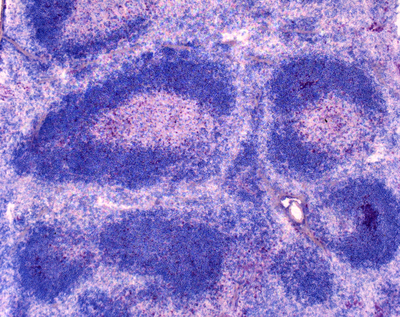
\includegraphics[scale=.72]{images/control.png} & 
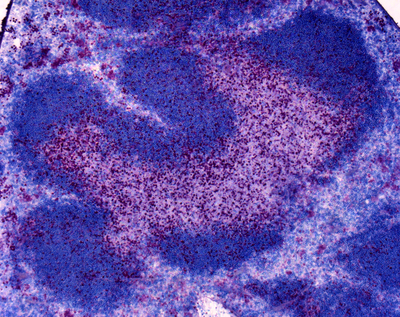
\includegraphics[scale=.72]{images/d3.png} & 
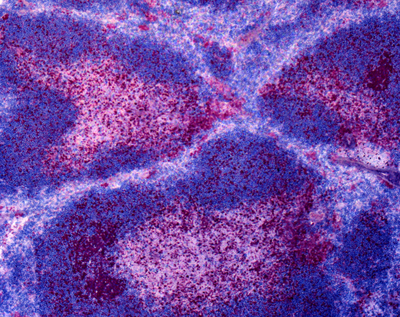
\includegraphics[scale=.72]{images/d4.png} \\
\end{tabular}

\begin{tabular}{lll}
	\s{d} \hspace{5cm} & \s{e} \\
	\multicolumn{2}{l}{\includegraphics[]{plots/histo.pdf}} & 
\end{tabular}

\begin{tabular}{l}
\s{f} \\
\includegraphics[]{plots/dge.pdf}
\end{tabular}


{\bfseries Figure 5: The CDR3$\beta$ repertoire desegregates despite ongoing immune response.} (a, b) TCZ segregation within (a) and between (b) mice reverts back to naïve-like levels at 4 days after SRBC challenge. (c) TCZs in a representative animal remain enlarged at d4 compared to naïve controls (B cells: blue; proliferating cells: red). (d) Cell proliferation in spleen remains ongoing at d4. (e) Germinal center formation begins at d4. (f) The three clones whose read counts in the blood differ most between na\"{i}ve and antigen-challenged mice (top row) also remain present in splenic TCZs at d4. Throughout, lines depict means and 95\% CIs.

\newpage



\newpage

\includegraphics[]{plots/permutation-test.pdf}

{\bfseries Supporting Figure 1: Recovering the origin of TCZ samples from mice as a validation of statistical repertoire analysis.} Biologically, one expects the repertoires from two TCZs in the same mouse to be more similar than from different mice. There are 15 possible ways to match 3 mice to 2 samples each. For each of these possibilities, the plots show the sum of the number of segregated clones (top row) or Jaccard indices (bottom row) for TCZ of the same mouse. Both segregation and the Jaccard index correctly recover the correct assignment. However, the difference between the correct assignments and incorrect ones is far more pronounced for the segregation method than for the Jaccard index.

\newpage


\includegraphics[page=3]{plots/usage-shared.pdf}

{\bfseries Supporting Figure 2: V- and J-segment usage of naïve CDR3$\beta$ repertoires compared to 3d after SRBC infection.}

\newpage


\includegraphics[page=3]{plots/fig4.pdf}

{\bfseries Supporting Figure 3: Analysis of the differences between the 20 most abundant clones in each TCZ at 4d after SRBC infection.}

\end{document}
